% Tento soubor nahraďte vlastním souborem s přílohami (nadpisy níže jsou pouze pro příklad)
% This file should be replaced with your file with an appendices (headings below are examples only)

% Umístění obsahu paměťového média do příloh je vhodné konzultovat s vedoucím
% Placing of table of contents of the memory media here should be consulted with a supervisor
%\chapter{Obsah přiloženého paměťového média}

%\chapter{Manuál}

%\chapter{Konfigurační soubor} % Configuration file

%\chapter{RelaxNG Schéma konfiguračního souboru} % Scheme of RelaxNG configuration file

%\chapter{Plakát} % poster


\chapter{PIR signal recording}
\label{appendix:PIRSignal}

The movements that data shows were prepared in several directions
and the type of movement can be read from the figure captions.

The trajectories are concentred circles with sensor in center and
radius values $3~m$, $6~m$, $9~m$ and $12~m$. The direction is
either left-to-right (LR) or right-to-left (RL).
\footnote{For example {\it 6m\_RL} is movement $6~m$ from sensor right-to-left.}
The movement was recorded multiple times.

Other cases are recorded as well: person walking towards ({\it C\_BF})
or walking away ({\it C\_FB}) from the sensor and no movement ({\it E}). 

\begin{figure}[!ht]
\begin{center}
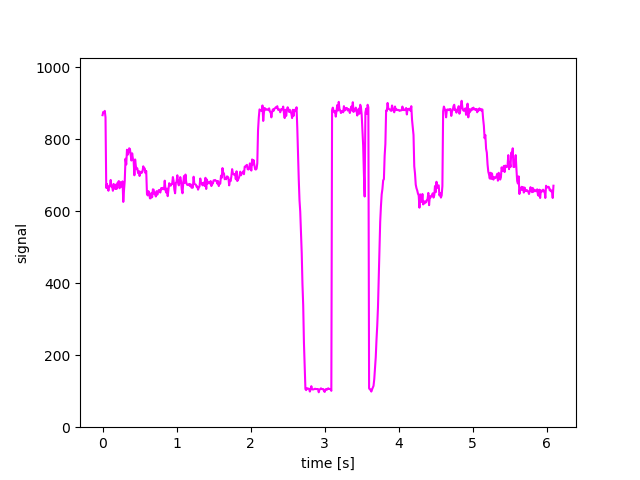
\includegraphics[width=0.3\textwidth]{../data/3m_LR/3m_LR_1.png}
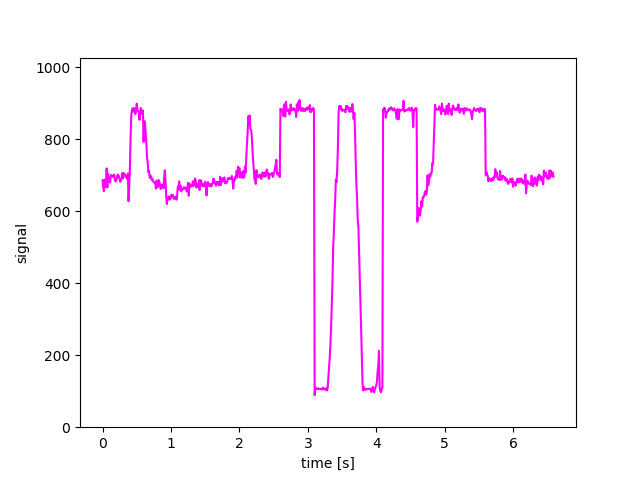
\includegraphics[width=0.3\textwidth]{../data/3m_LR/3m_LR_2.png}
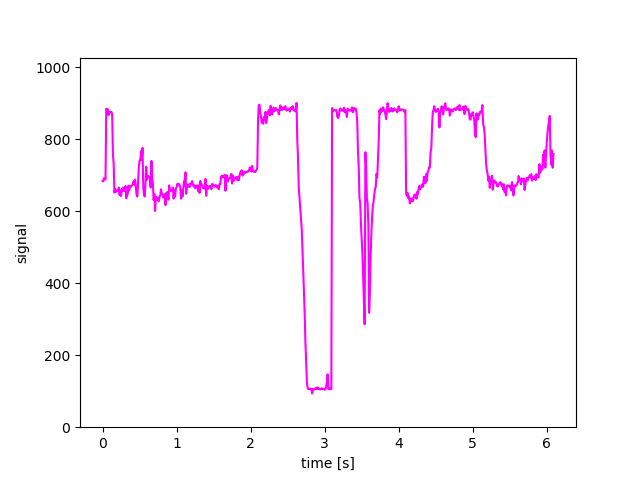
\includegraphics[width=0.3\textwidth]{../data/3m_LR/3m_LR_3.png}
\caption{3m\_LR.\label{fig:3m_LR}}
\end{center}
\end{figure}

\begin{figure}[!ht]
\begin{center}
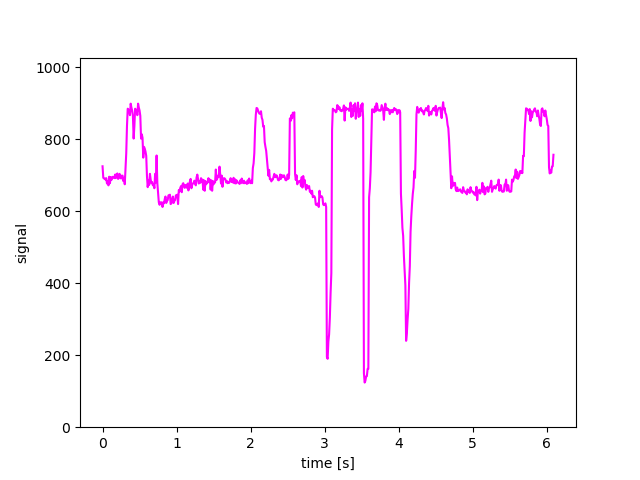
\includegraphics[width=0.3\textwidth]{../data/3m_RL2/3m_RL2_1.png}
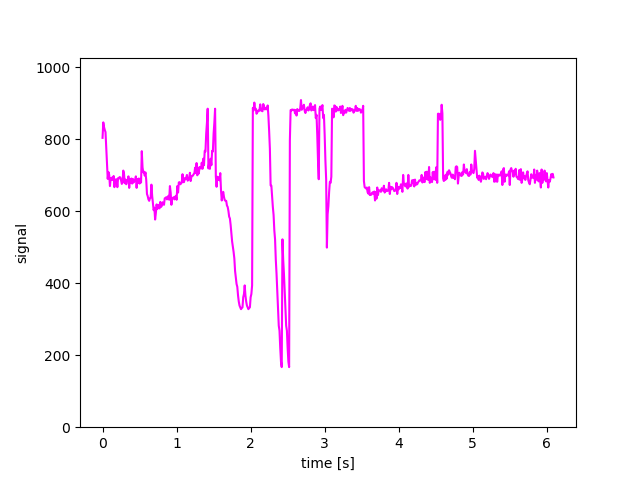
\includegraphics[width=0.3\textwidth]{../data/3m_RL2/3m_RL2_2.png}
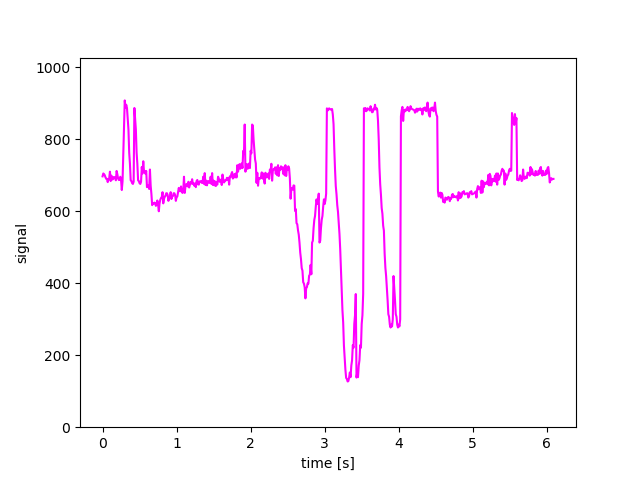
\includegraphics[width=0.3\textwidth]{../data/3m_RL2/3m_RL2_3.png}
\caption{3m\_RL.\label{fig:3m_RL}}
\end{center}
\end{figure}

\begin{figure}[!ht]
\begin{center}
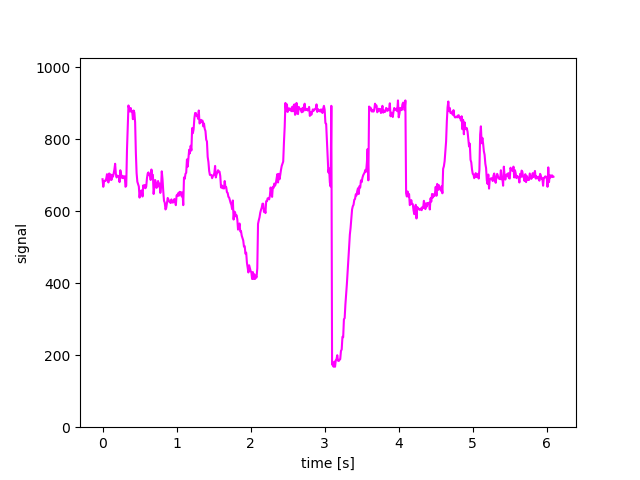
\includegraphics[width=0.3\textwidth]{../data/6m_LR/6m_LR_1.png}
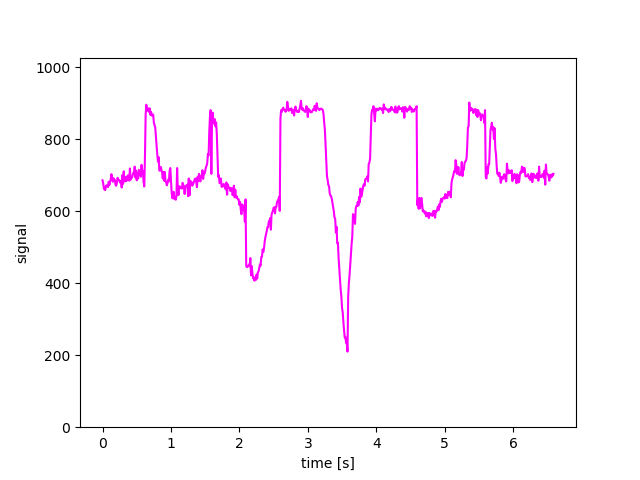
\includegraphics[width=0.3\textwidth]{../data/6m_LR/6m_LR_2.png}
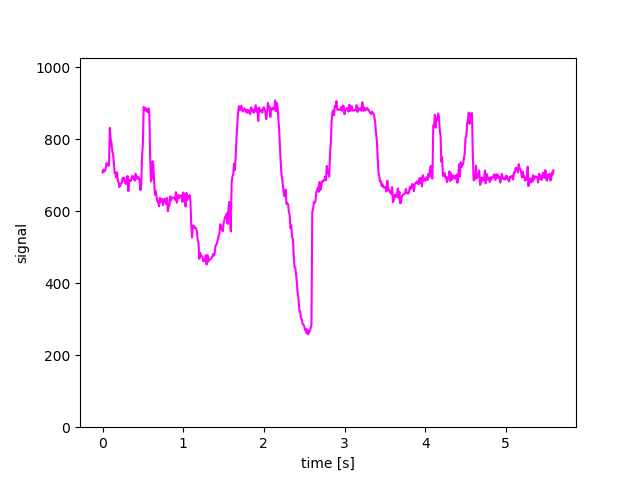
\includegraphics[width=0.3\textwidth]{../data/6m_LR/6m_LR_3.png}
\caption{6m\_LR.\label{fig:6m_LR}}
\end{center}
\end{figure}

\begin{figure}[!ht]
\begin{center}
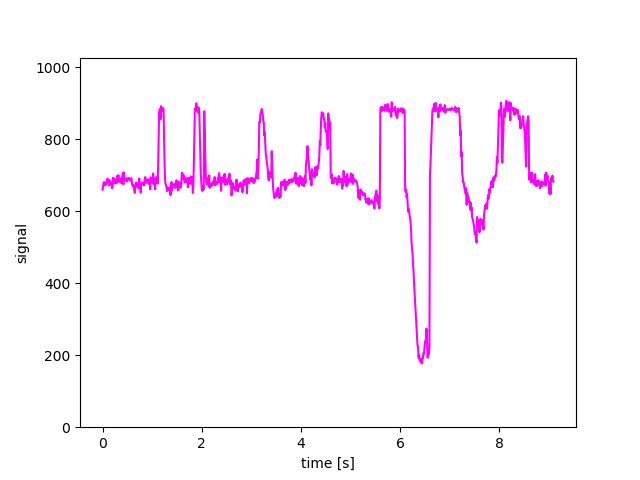
\includegraphics[width=0.3\textwidth]{../data/6m_RL/6m_RL_1.png}
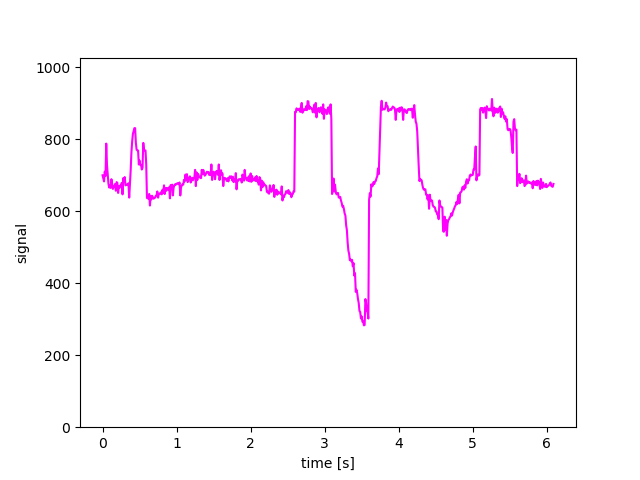
\includegraphics[width=0.3\textwidth]{../data/6m_RL/6m_RL_2.png}
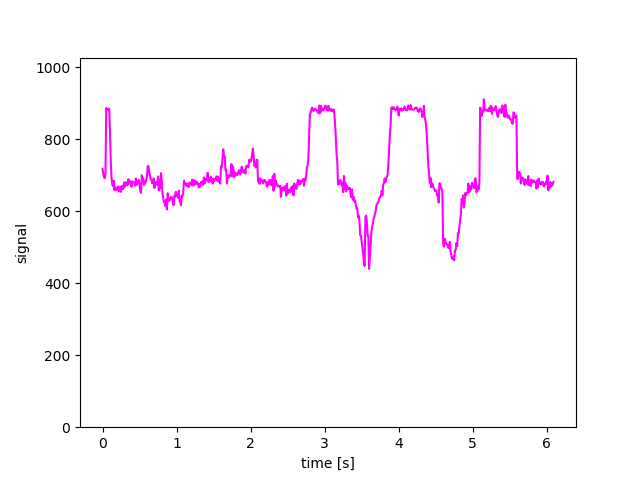
\includegraphics[width=0.3\textwidth]{../data/6m_RL/6m_RL_3.png}
\caption{6m\_RL.\label{fig:6m_RL}}
\end{center}
\end{figure}


\begin{figure}[!ht]
\begin{center}
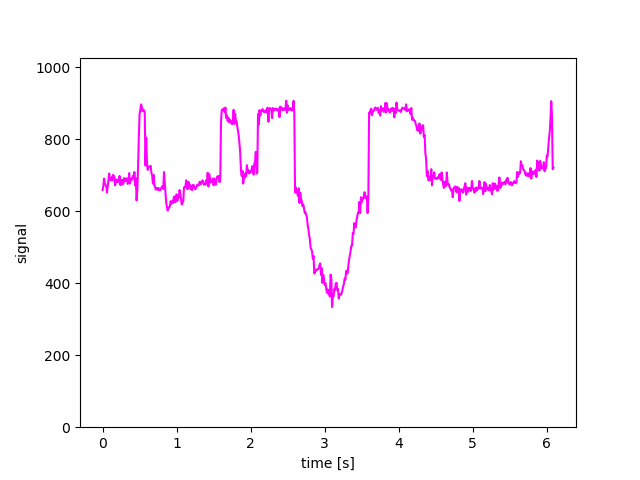
\includegraphics[width=0.32\textwidth]{../data/9m_LR/9m_LR_1.png}
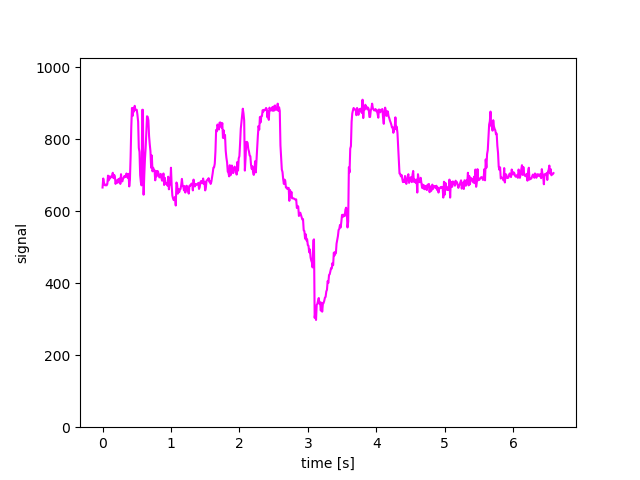
\includegraphics[width=0.32\textwidth]{../data/9m_LR/9m_LR_2.png}
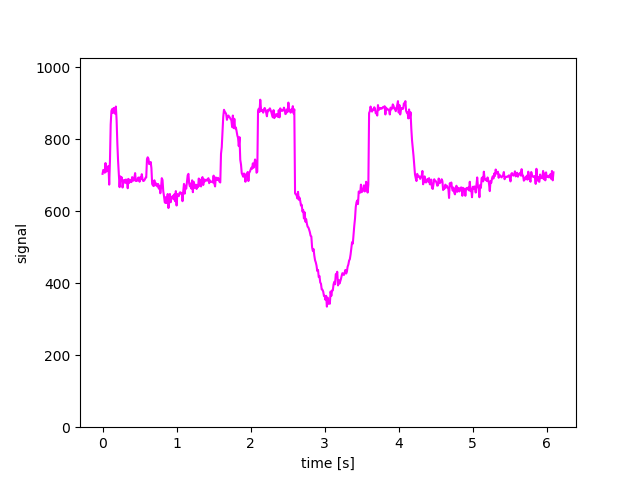
\includegraphics[width=0.32\textwidth]{../data/9m_LR/9m_LR_3.png}
\caption{9m\_LR.\label{fig:9m_LR}}
\end{center}
\end{figure}

\begin{figure}[!ht]
\begin{center}
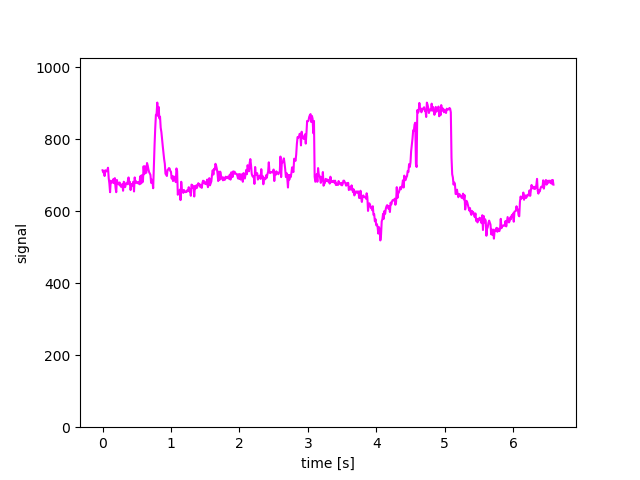
\includegraphics[width=0.3\textwidth]{../data/9m_RL/9m_RL_1.png}
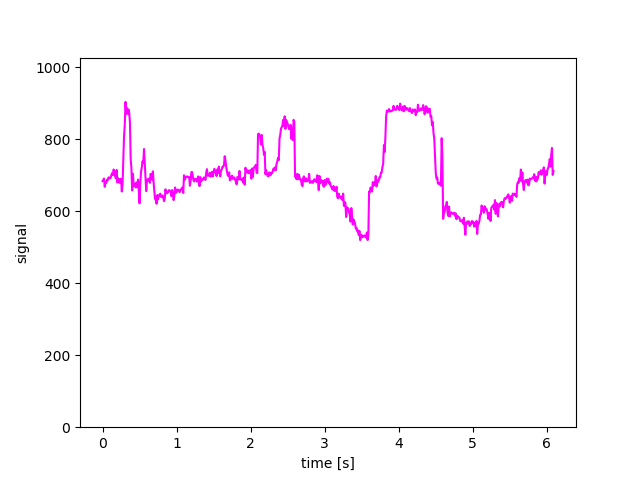
\includegraphics[width=0.3\textwidth]{../data/9m_RL/9m_RL_2.png}
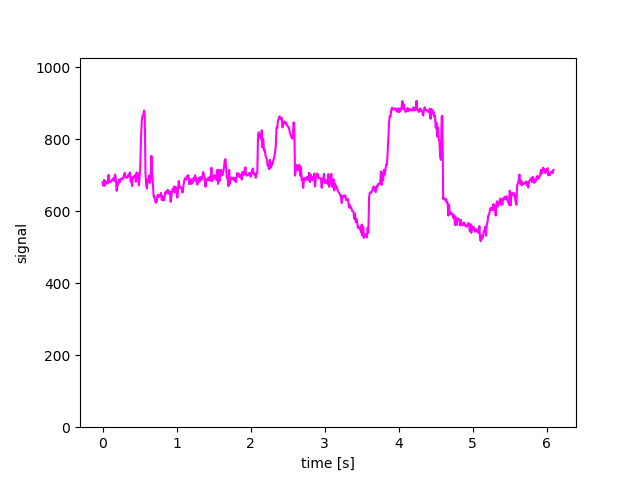
\includegraphics[width=0.3\textwidth]{../data/9m_RL/9m_RL_3.png}
\caption{9m\_RL.\label{fig:9m_RL}}
\end{center}
\end{figure}

\begin{figure}[!ht]
\begin{center}
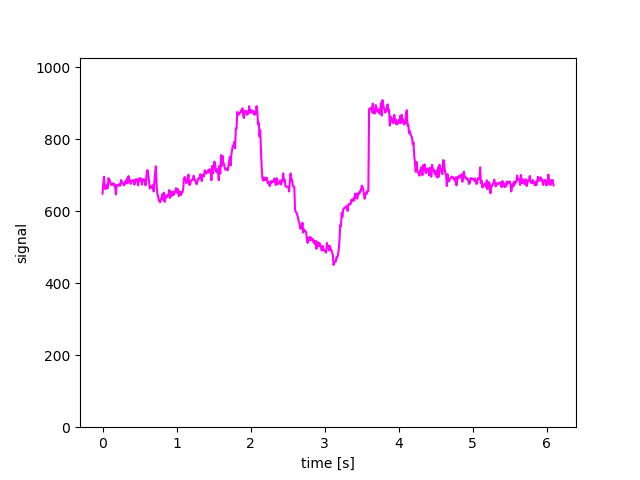
\includegraphics[width=0.3\textwidth]{../data/12m_LR/12m_LR_1.png}
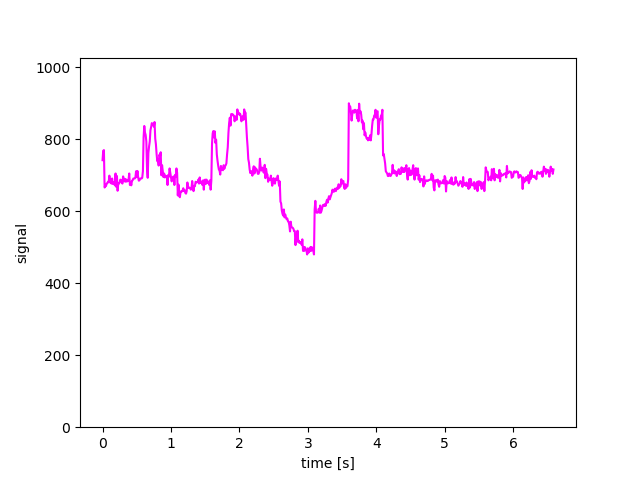
\includegraphics[width=0.3\textwidth]{../data/12m_LR/12m_LR_2.png}
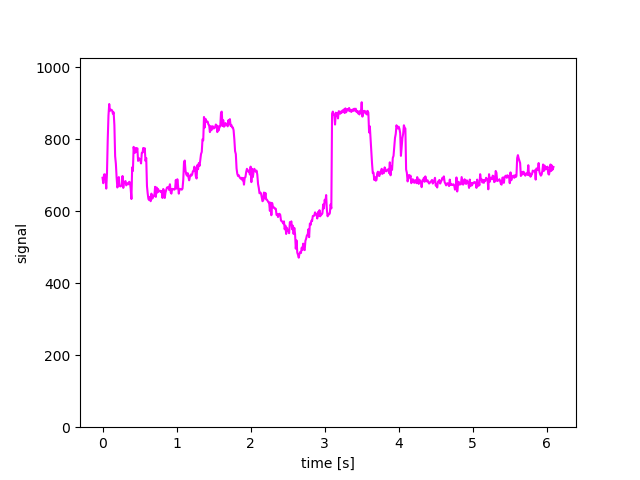
\includegraphics[width=0.3\textwidth]{../data/12m_LR/12m_LR_3.png}
\caption{12m\_LR.\label{fig:12m_LR}}
\end{center}
\end{figure}

\begin{figure}[!ht]
\begin{center}
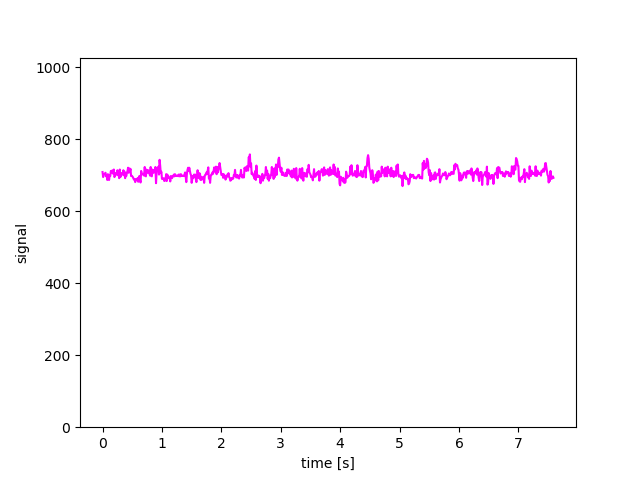
\includegraphics[width=0.3\textwidth]{../data/C_BF/C_BF_1.png}
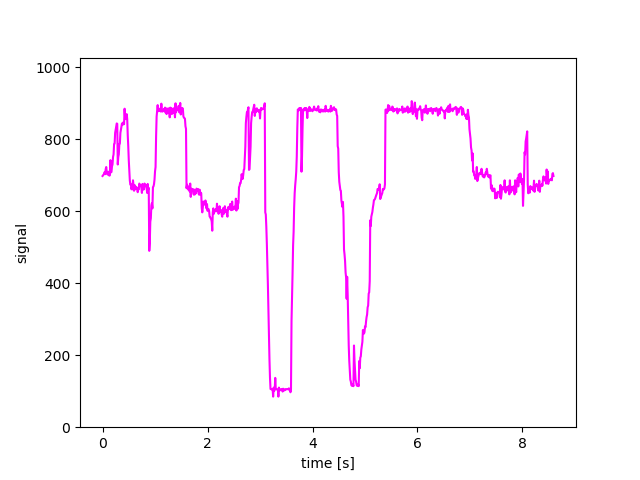
\includegraphics[width=0.3\textwidth]{../data/C_BF/C_BF_2.png}
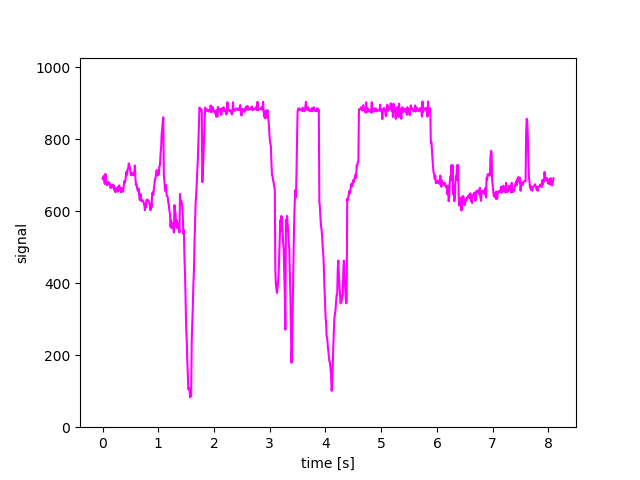
\includegraphics[width=0.3\textwidth]{../data/C_BF/C_BF_3.png}
\caption{C\_BF.\label{fig:C_BF}}
\end{center}
\end{figure}

\begin{figure}[!ht]
\begin{center}
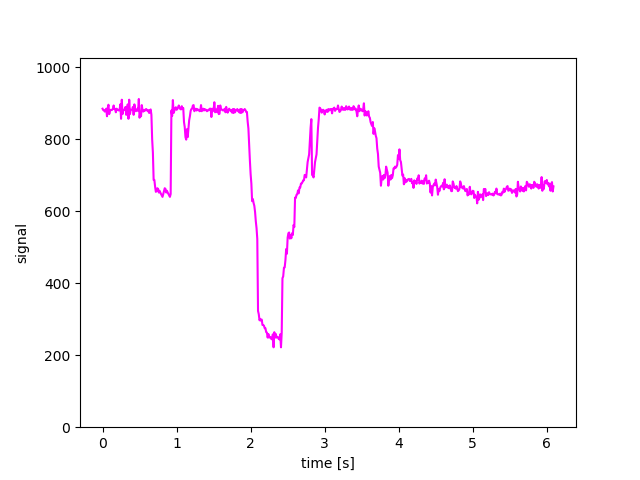
\includegraphics[width=0.3\textwidth]{../data/C_FB/C_FB_2.png}
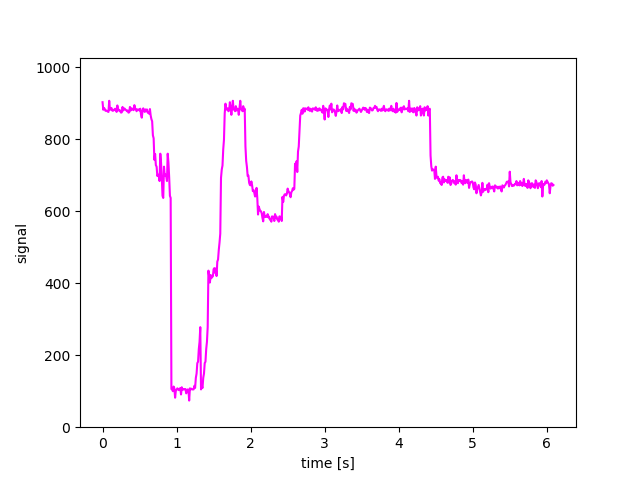
\includegraphics[width=0.3\textwidth]{../data/C_FB/C_FB_3.png}
\caption{C\_FB.\label{fig:C_FB}}
\end{center}
\end{figure}

\begin{figure}[!ht]
\begin{center}
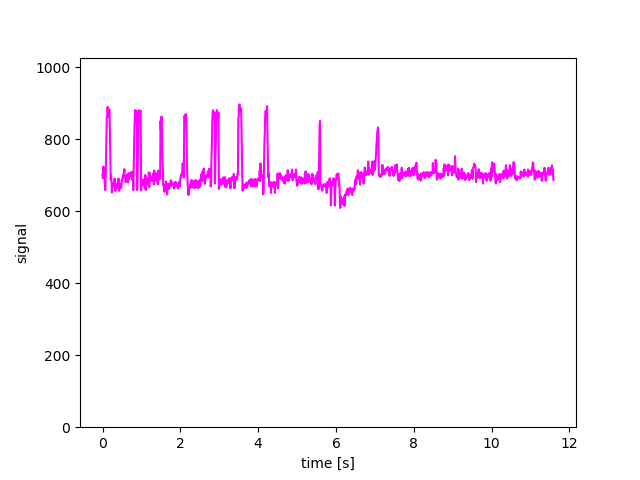
\includegraphics[width=0.3\textwidth]{../data/E2/E2_1.png}
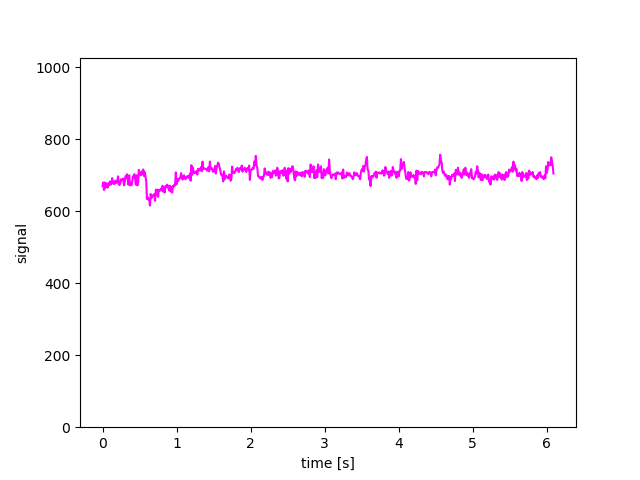
\includegraphics[width=0.3\textwidth]{../data/E2/E2_2.png}
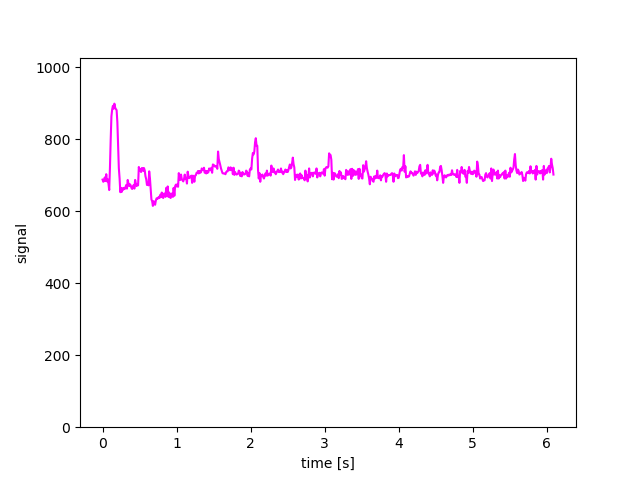
\includegraphics[width=0.3\textwidth]{../data/E2/E2_3.png}
\caption{E.\label{fig:C_FB}}
\end{center}
\end{figure}





